% ******************************************************** %
%              TEMPLATE DE INFORME ORGA2 v0.1              %
% ******************************************************** %
% ******************************************************** %
%                                                          %
% ALGUNOS PAQUETES REQUERIDOS (EN UBUNTU):                 %
% ========================================
%                                                          %
% texlive-latex-base                                       %
% texlive-latex-recommended                                %
% texlive-fonts-recommended                                %
% texlive-latex-extra?                                     %
% texlive-lang-spanish (en ubuntu 13.10)                   %
% ******************************************************** %


\documentclass[a4paper]{article}
\usepackage[spanish]{babel}
\usepackage[utf8]{inputenc}
\usepackage{charter}   % tipografia
\usepackage{graphicx}
%\usepackage{makeidx}
\usepackage{paralist} %itemize inline

%\usepackage{float}
%\usepackage{amsmath, amsthm, amssymb}
%\usepackage{amsfonts}
%\usepackage{sectsty}
%\usepackage{charter}
%\usepackage{wrapfig}
%\usepackage{listings}
%\lstset{language=C}

% \setcounter{secnumdepth}{2}
\usepackage{underscore}
\usepackage{caratula}
\usepackage{url}
\usepackage[document]{ragged2e}
\usepackage[export]{adjustbox}
\usepackage{subcaption}
\usepackage{floatrow}


% ********************************************************* %
% ~~~~~~~~              Code snippets             ~~~~~~~~~ %
% ********************************************************* %

\usepackage{color} % para snipets de codigo coloreados
\usepackage{fancybox}  % para el sbox de los snipets de codigo

\definecolor{litegrey}{gray}{0.94}

\newenvironment{codesnippet}{%
	\begin{Sbox}\begin{minipage}{\textwidth}\sffamily\small}%
	{\end{minipage}\end{Sbox}%
		\begin{center}%
		\vspace{-0.4cm}\colorbox{litegrey}{\TheSbox}\end{center}\vspace{0.3cm}}



% ********************************************************* %
% ~~~~~~~~         Formato de las páginas         ~~~~~~~~~ %
% ********************************************************* %

\usepackage{fancyhdr}
\pagestyle{fancy}

%\renewcommand{\chaptermark}[1]{\markboth{#1}{}}
\renewcommand{\sectionmark}[1]{\markright{\thesection\ - #1}}

\fancyhf{}

\fancyhead[LO]{Sección \rightmark} % \thesection\ 
\fancyfoot[LO]{\small{Luis Enrique Badell Porto, Nicolas Bukovits, Kevin Frachtenberg}}
\fancyfoot[RO]{\thepage}
\renewcommand{\headrulewidth}{0.5pt}
\renewcommand{\footrulewidth}{0.5pt}
\setlength{\hoffset}{-0.8in}
\setlength{\textwidth}{16cm}
%\setlength{\hoffset}{-1.1cm}
%\setlength{\textwidth}{16cm}
\setlength{\headsep}{0.5cm}
\setlength{\textheight}{25cm}
\setlength{\voffset}{-0.7in}
\setlength{\headwidth}{\textwidth}
\setlength{\headheight}{13.1pt}

\renewcommand{\baselinestretch}{1.1}  % line spacing

% ******************************************************** %


\begin{document}


\thispagestyle{empty}
\materia{Organización del Computador II}
\submateria{Primer Cuatrimestre de 2016}
\titulo{Trabajo Práctico 2}
\subtitulo{Procesamiento de imágenes con SIMD}
\integrante{Luis Enrique Badell Porto}{246/13}{luisbadell@gmail.com}
\integrante{Nicolas Bukovits}{546/14}{nicko_buk@hotmail.com}
\integrante{Kevin Frachtenberg}{247/14}{kevinfra94@gmail.com}
\grupo{Grupo: Yo no manejo el raiting, yo manejo un Rolls-Royce}
\maketitle

%{\small\textbf{\flushleft{Resumen}}\\
\abstract {En el siguiente trabajo pr\'actico, se busca analizar, estudiar y comprender el funcionamiento y rendimiento de la tecnolog\'ia
SIMD (Single Instruction Multiple Data) inclu\'ida en el sistema SSE de los procesadores Intel. Para esto, se realizaron tres filtros
de im\'agenes (Cropflip, Sepia y Low Dynamic Range) en lenguaje C y en lenguaje ensamblador para aplicar sobre imagenes BMP, y luego se comparó el rendimiento entre ellos.
Los resultados obtenidos de estos experimentos, fueron plasmados y analizados en este informe.
}

%\newpage

%\thispagestyle{empty}
%\vfill


\thispagestyle{empty}
\vspace{3cm}
\tableofcontents
\newpage


%\normalsize
\newpage



\section{Introduccion}
\subsection{Cropflip}
El filtro cropflip recibe como parametros extra dos tamaños y dos offset. Un tamaño y un offset para las filas, y los otros dos para las columnas.
Lo que se hace con esto es recortar la imagen original en una nueva imagen e invertirla verticalmente. La imagen se recorta desde
donde los offsets lo indican hasta el tamaño indicado.
\newline 
Ejemplo: cropflip lena32.bmp 128 128 40 50 

\begin{figure}[!ht]
    \centering
    \begin{floatrow}
      \ffigbox[\FBwidth]{\caption{Antes del filtro cropflip}}{%
        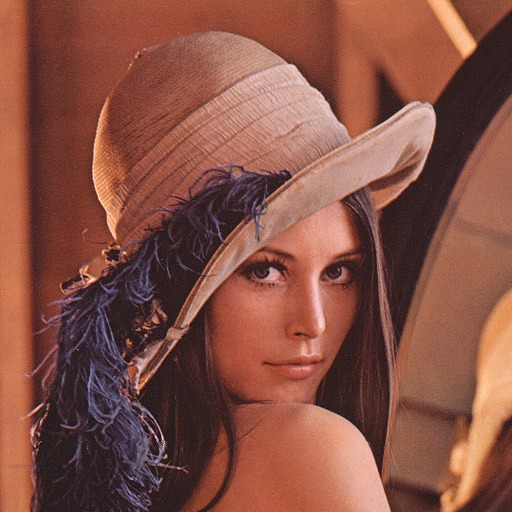
\includegraphics[scale=.25]{./imagenes/lena32.jpg}   
      }
      \ffigbox[\FBwidth]{\caption{Después del filtro cropflip}}{%
       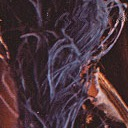
\includegraphics[scale=.5]{./imagenes/lena32-cropflip.jpg} 
      }
    \end{floatrow}
\end{figure}

Para el caso de la implementación en lenguaje C, se toma pixel por pixel y se copia al lugar correspondiente (invirtiendo la imagen)
en la imagen destino.
Por otro lado, en el caso de la implementación en lenguaje ensamblador, se utilizan los registros XMM para leer y copiar de a 4 pixels
en la imagen final.

\subsection{Sepia}
El filtro sepia, es el conocido filtro de imagenes que simula una foto antigüa. Para lograr este efecto, lo que se hace es una suma
de los canales de color (R, G, B. Llamaremos a esta suma "SumaRGB") y luego se multiplica por un valor fijo para cada canal (0.5 para el canal R, 0.3 para el G
y 0.2 para el canal B). Luego, manteniendo la transparencia en caso de haber, el pixel quedaría conformado por A = A, R = SumaRGB*0.5
, G = SumaRGB*0.3 y B = SumaRGB*0.2. \newline
Al igual que en Cropflip, en el caso de C, se trabaja pixel por pixel, mientras que en el caso del lenguaje ensamblador se trabaja un poco diferente:
Si bien se lee de a 4 pixeles de la imagen original, luego es necesario trabajar pixel por pixel ya que cada canal tiene un tamaño de 1 byte
y si quisiéramos realizar la suma de los 3 canales de los 4 pixeles en un solo registro, ésta no entraría en un byte. De esta forma, lo que se hace
es expandir (unpack) cada pixel para que cada canal pase a tener un tamaño de word (2 bytes). Así, la suma máxima será de 255 + 255 + 255, y esto sí
entra en un espacio de tamaño word. Sin embargo, las instrucciones que provee el procesador Intel para multiplicar por floats, nos obliga
a realizar otra expanción (unpack) de cada pixel, pero esta vez de word a Double word (4 bytes, mismo tamaño que un float).
Una vez están listos los cálculos de cada uno de los 4 pixels, se realizan 2 packs para llevar cada canal de doubleword a byte nuevamente.
\newline
Ejemplo: sepia foto.bmp
\begin{figure}[!ht]
    \centering
    \begin{floatrow}
      \ffigbox[\FBwidth]{\caption{Antes del filtro sepia}}{%
        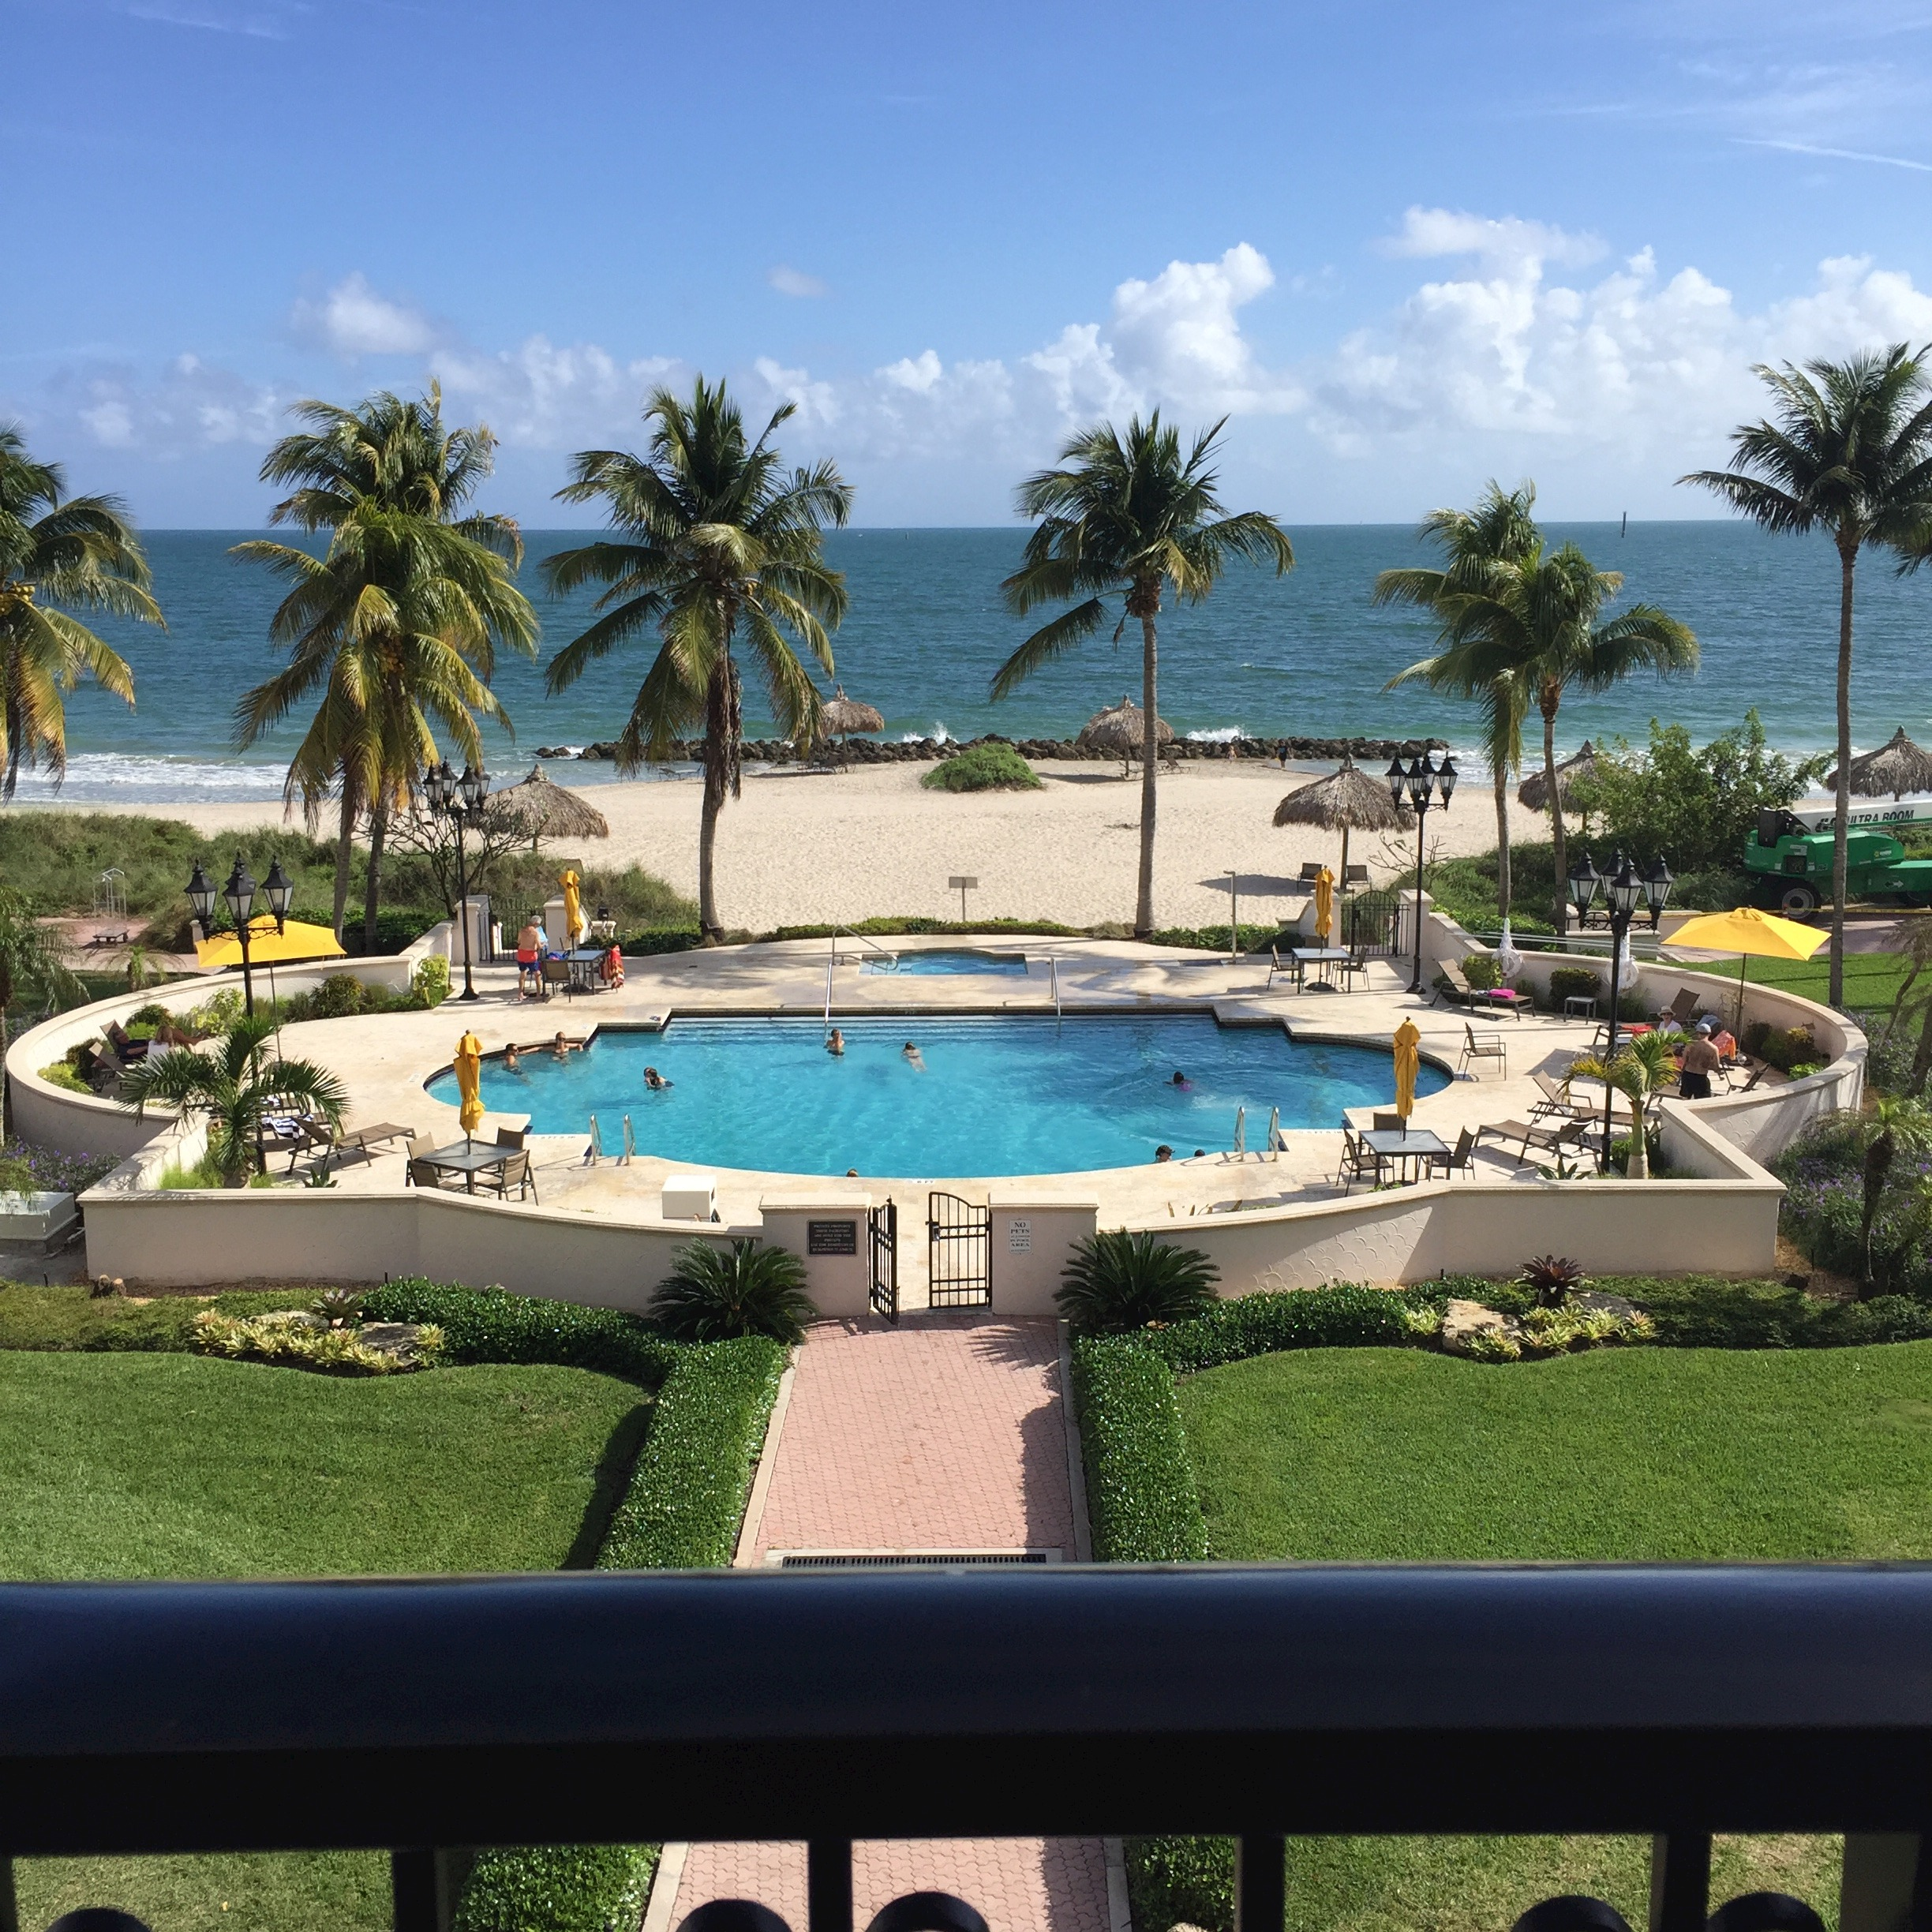
\includegraphics[scale=.04]{./imagenes/foto.jpg}   
      }
      \ffigbox[\FBwidth]{\caption{Después del filtro sepia}}{%
       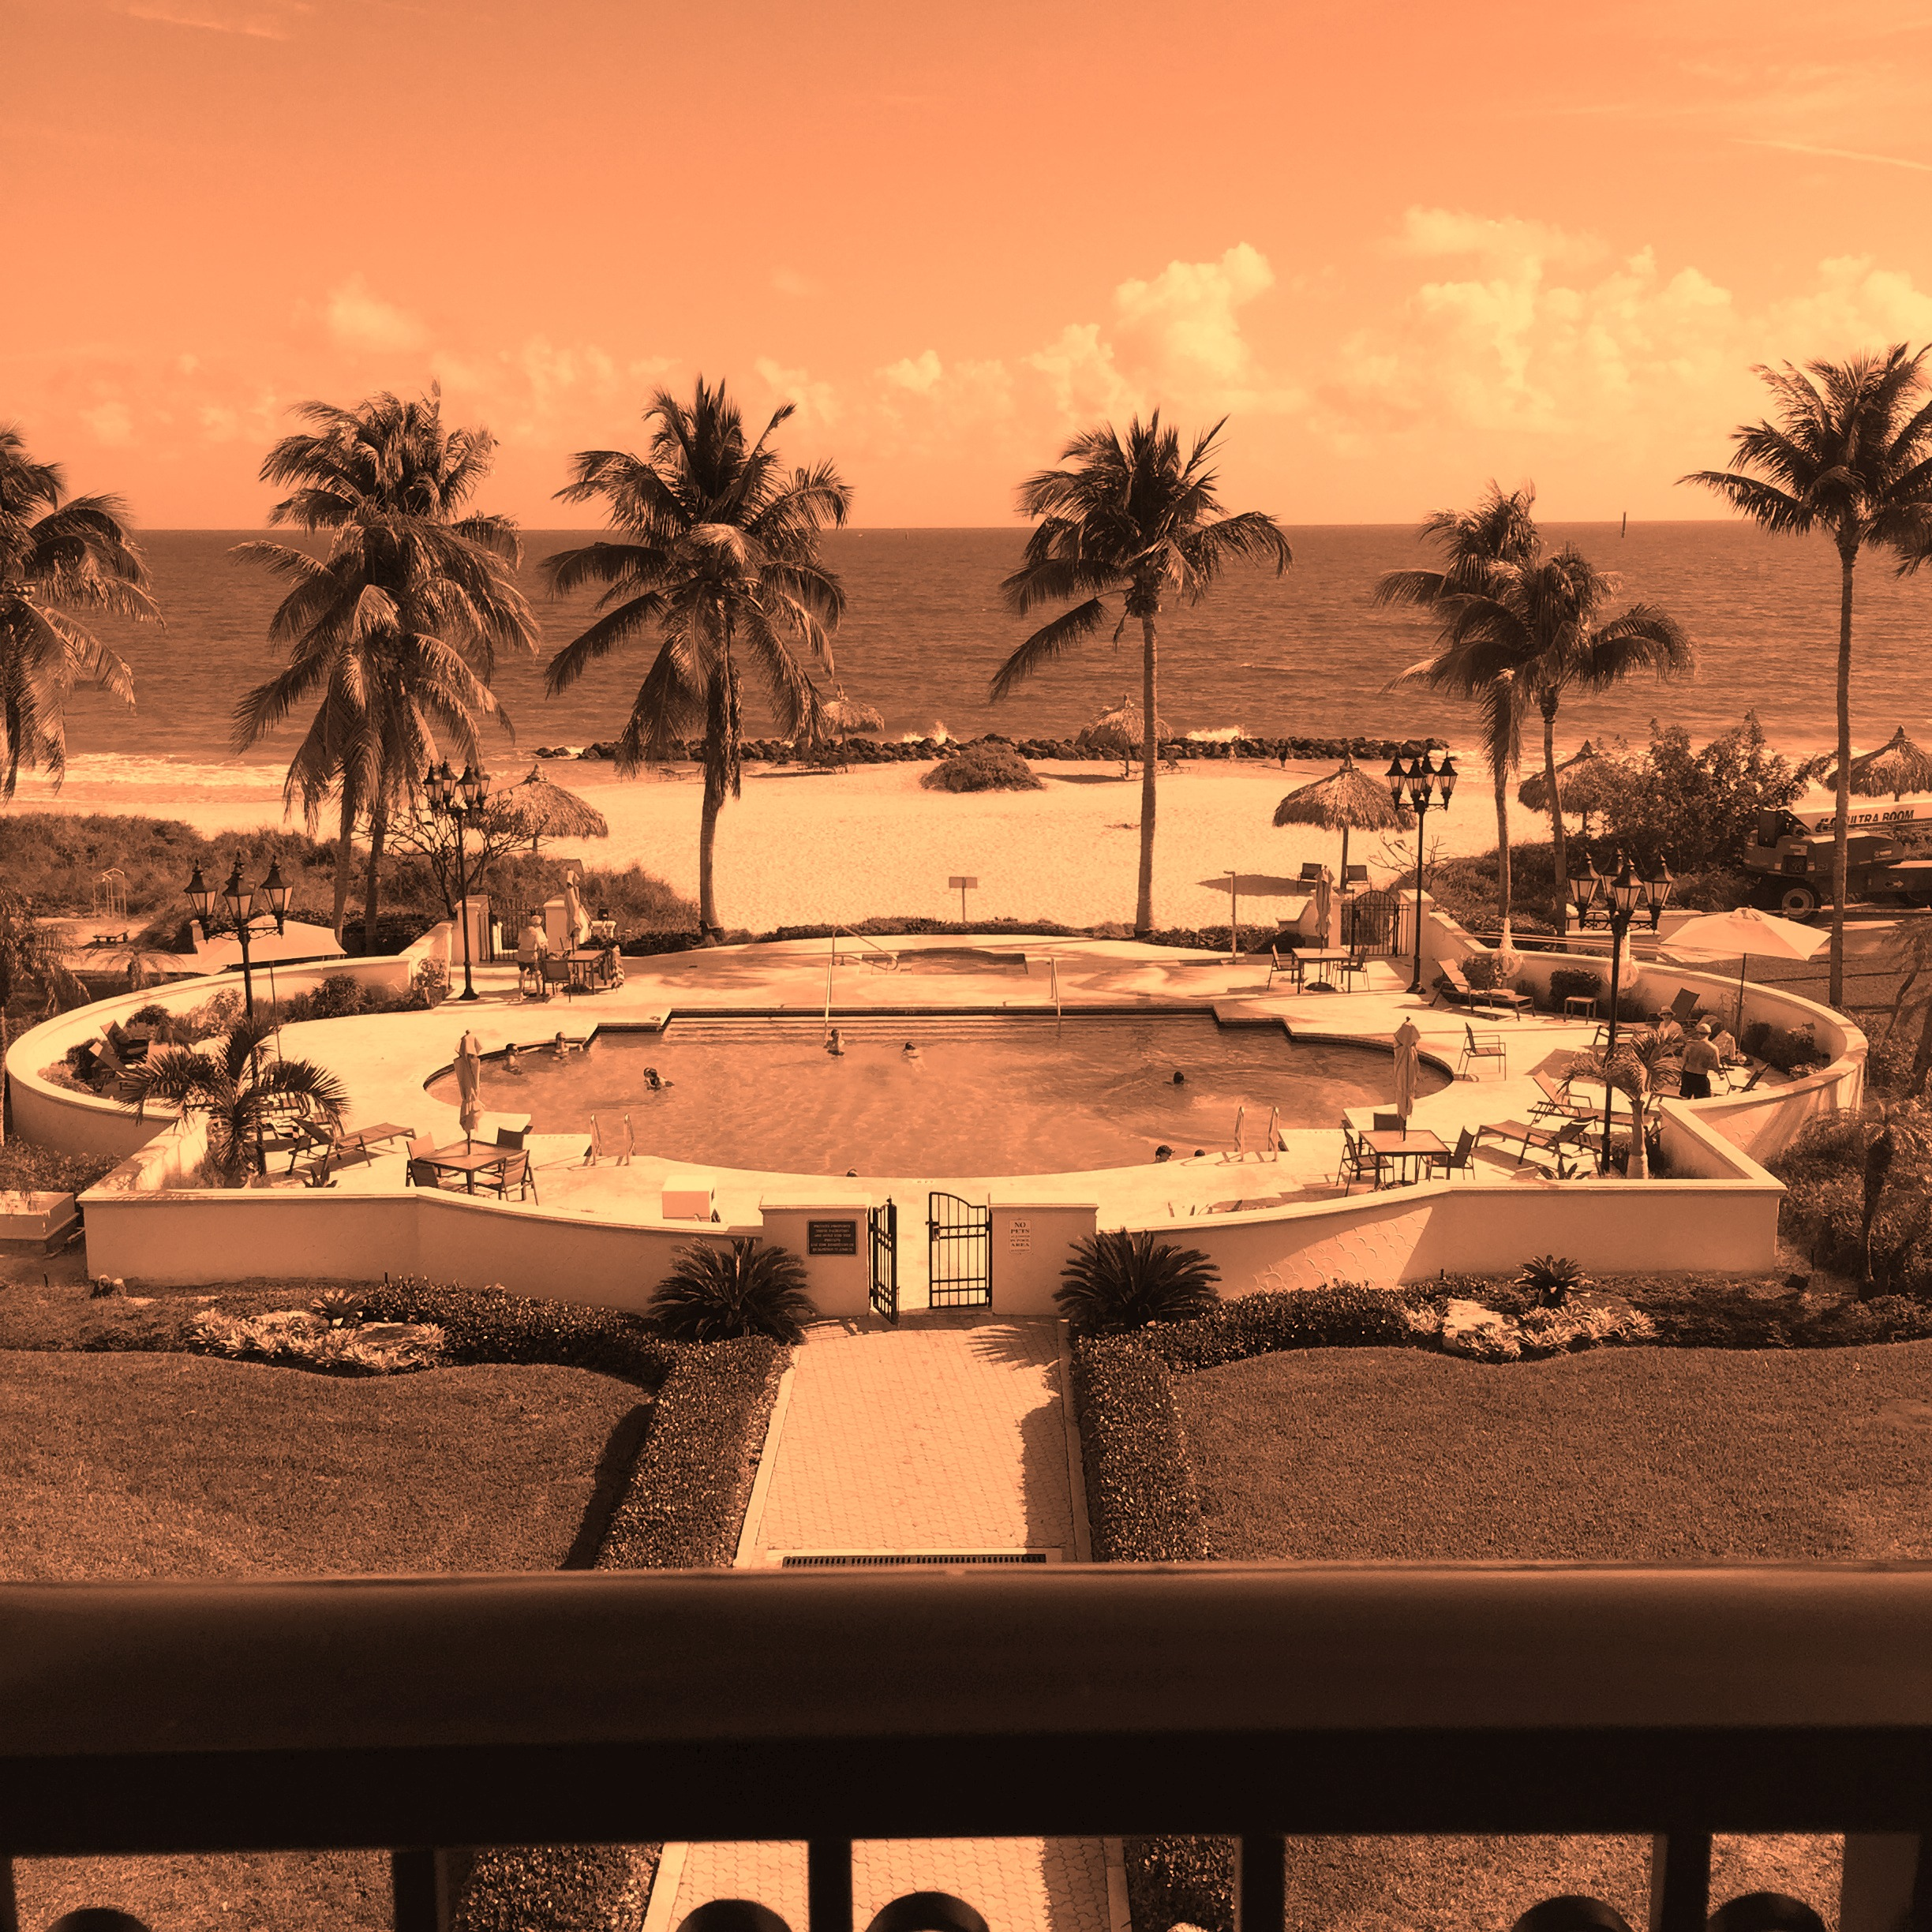
\includegraphics[scale=.04]{./imagenes/foto-sepia.jpg} 
      }
    \end{floatrow}
\end{figure}

\subsection{Low Dynamic Range}
Este filtro, más conocido como LDR, se logra realizando una serie de cálculos en base a los 25-vecinos de cada pixel del interior
de la imagen (si tomamos "interior" como 2 pixels hacia adentro desde cada borde) y un $\alpha$ pasado por parámetro, el cual puede ser
un valor entre -255 y 255. Lo que hace es agregar o quitar luminosidad dependiendo de este $\alpha$. El método para lograr este efecto es
modificar cada canal de color (R,G,B) del pixel a revisar, a través de realizar una suma de los 3 canales de color de los 25-vecinos del pixel a editar (incluyendo el mismo pixel),
luego se multiplica ese valor por el $\alpha$ y por el valor del canal del pixel en observación. Por último, se divide por un valor "Max",
que se da haciendo el cálculo del posible máximo del cálculo anterior (255*25*3*255), se suma el valor del canal antes multiplicado y antes
de guardarse, se satura a 0 y 255, que es el maximo de cada canal (ya que como el $\alpha$ puede ser negativo, es necesario tomar el caso
en que quede un número negativo en el canal).
\newline
El caso de C es igual a sepia y cropflip: Se analiza pixel por pixel. El caso del lenguaje ensamblador es parecido, ya que no se pueden
hacer cálculos tan grandes con 4 pixeles al mimso tiempo. Es por esto, que también se analiza pixel por pixel, pero para realizar el
cálculo de la suma de los 25 vecinos, las multiplicaciones, la división, suma y saturación, se utilizan instrucciones SSE.
\newline
Ejemplo: ldr bob.bmp 100
\begin{figure}[!ht]
    \centering
    \begin{floatrow}
      \ffigbox[\FBwidth]{\caption{Antes del filtro ldr}}{%
        
\includegraphics[scale=.25]{./imagenes/bob.jpg}   
      }
      \ffigbox[\FBwidth]{\caption{Después del filtro ldr}}{%
       
\includegraphics[scale=.25]{./imagenes/bob-ldr.jpg} 
      }
    \end{floatrow}
\end{figure}


\section{Desarrollo}

\subsection{Hipótesis y bases}
Nosotros tenemos como hipótesis que dadas las herramientas que nos ofrece la tecnología SSE, y que nosotros mismos somos los que nos
ocupamos de hacer una buena implementación en cada lenguaje, los algoritmos hechos en lenjuage ensamblador será mucho más rápido
que los que están hechos en lenguaje C. Sabemos que parte del retraso que tiene el lenguaje C se debe a que es el compilador quien decidirá cómo
optimizar el algoritmo implementado; esto es, traducir a código de máquina según la interpretación que le de el copmilador al código C. Es por esto 
que usaremos el flag O3 como caso de compilación extra, y así poder comparar distintos métodos de compilación sobre una misma 
implementación del lenguaje C.
En cambio, para el caso del lenjuage ensamblador, es simplemente traducir a código de máquina, ya que son directamente las instrucciones
que el procesador deberá ejecutar.
\newline
Para poder comparar cada implementación de los filtros, los mismos se ejecután reiteradas veces en imagenes de distintos tamaños.
De cada ejecución, tomaremos el tiempo del clock antes de correr el programa y después de correrlo, y además observaremos
la cantidad de ciclos de reloj que toma cada vez. Si bien esto puede traer problemas como por ejemplo el tema de los \textit{outliers},
por razones de probabilidad y estadística, un promedio de cantidades grandes se acercará más a un promedio real.

\subsection{Implementación y Análisis}

\subsubsection{Cropflip}
Como se mencionó en la introducción, el filtro de Cropflip toma, en el caso de C, cada pixel y se copia de memoria a memoria. 
Sabemos que en la práctica esto solo funciona con un DMA, por lo que depende del compilador decidir cómo hacer las iteraciones para 
recorrer la imagen original y copiar cada pixel a la nueva posición de memoria.
Para el caso de ASM, se toma de a 4 pixels y se mueven a un registro XMM. dado que un pixel tiene tamaño de 64 bits y el tamaño
del registro XMM es de 128, hacer esto es posible mediante instrucciones SSE (en este caso, movdqu). Luego lo mueve nuevamente a memoria
en la posición correspondiente para ese pixel en la nueva imagen. 
Para este filtro, los tests que se realizados consideraron distintos offsets y tamaños de imágenes, además de realizarse sobre imágenes de
distintos tamaños. 
\newline
Los parámetros utilizados para esta experimentación fueron tamx: 128, tamy: 128, offsetx: i-128, offsety: i-128. Donde \textit{i} es
el tamaño de un lado de la imagen, que al ser cuadradas y múltiplos de 4, hace que sea indiferente el lado a elegir.
Este Offset permite tener en cuenta el desplazamiento que debe realizarse para empezar a copiar la imagen, el cual es hasta el último
bloque de 128x128 de la imagen original.
\newline
El primer caso de comparación es la implementación en C compilado sin el Flag O3 contra la implementación en ASM. En el siguiente gráfico
se puede observar la diferencia de tiempo de cada implementación en ciclos de reloj sobre el tamaño de la imagen en pixels.

\begin{figure}[!ht]
    \centering
    \begin{floatrow}
      \ffigbox[\FBwidth]{\caption{Comparación C sin optimizar vs ASM}}{%
        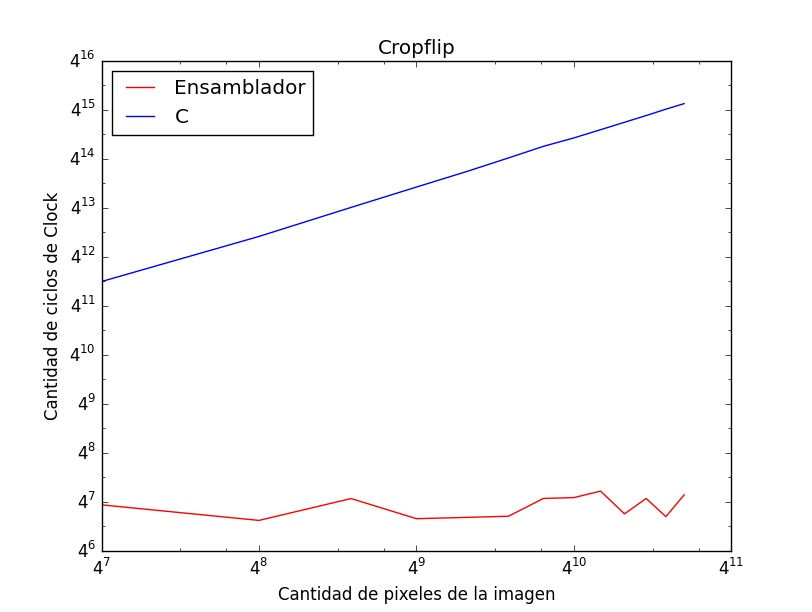
\includegraphics[scale=.25]{./imagenes/cropflip-asmVSc.jpg}   
      }
    \end{floatrow}
\end{figure}

Podemos bbservar de este experimento que la implementación en C es que si bien está basada en la misma idea que la implementación en ASM,
el código generado por el compilador hace que tome mucho más tiempo resolver cada aplicación del filtro hasta el punto de crecer linealmente
respecto del tamaño de la imágen. Podemos entender esto como una muestra de la diferencia en capacidad de procesamiento de los procesadores que utilizan
la tecnología SSE contra los que no la utilizan o tienen.

\begin{figure}[!ht]
    \centering
    \begin{floatrow}
      \ffigbox[\FBwidth]{\caption{Comparación C con optimización O3 vs ASM}}{%
        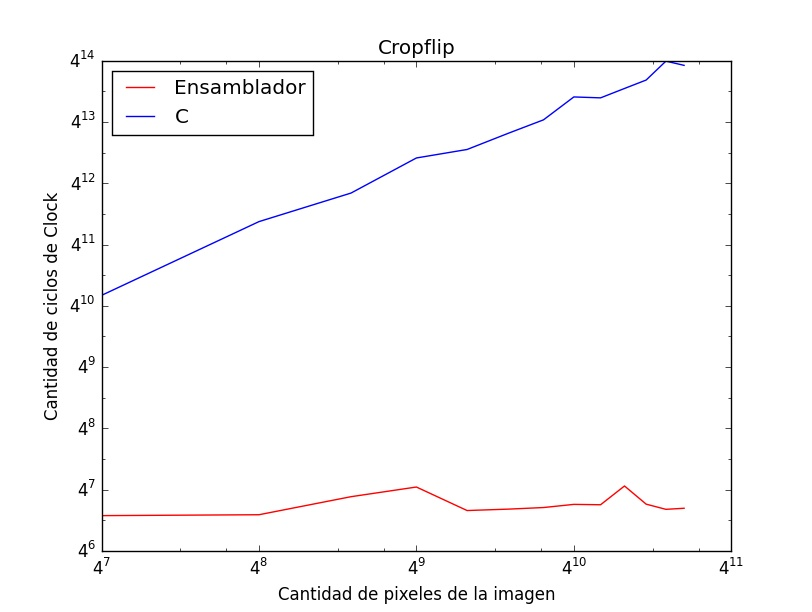
\includegraphics[scale=.25]{./imagenes/cropflip-asmVScO3.jpg}   
      }
    \end{floatrow}
\end{figure}

En este segundo experimento, comparamos la misma implementación C que el caso anterior pero esta vez compilado con el flag O3, 
el cual permite compilar el código utilizando tecnología SSE...

\subsubsection{Sepia}


\section{Conclusiones y trabajo futuro}






%\begin{codesnippet}
%\begin{verbatim}

%struct Pepe {

 %   ...

%};

%\end{verbatim}
%\end{codesnippet}

\end{document}

